In this chapter we first discuss our Facebook Link Recommendation
(LinkR) application and then proceed to discuss how it can be
evaluated using general principles of evaluation used in the
machine learning and information retrieval fields.

\subsection{Facebook}

Facebook is a social networking service that is currently the largest
in the world. As of July 2011 it had more that 750 million active
users. Users in Facebook create a profile and establish ``friend''
connections between users to establish their social network. Each user
has a ``Wall'' where they and their friends can make posts to.  These
posts can be links, photos, status updates, etc.  Items that have been
posted by a user can be ``liked'', shared, or commented upon by other
users.  An example of a link post on a Wall that had been liked
by others was provided previously in Figure~\ref{fig:ex_link}.

%\begin{figure}[h]
%\centering
%\subfigure{
\includegraphics[scale=0.50]{img/posted-link.png}}
%\subfigure{
\includegraphics[scale=0.50]{img/posted-link.eps}}
%\caption{A link posted by the author that has been liked by three other users.}
%\end{figure}

This thesis seeks to find out how best to recommend links to
individual users such that there is a high likelihood that they will
``like'' their recommended links.  We do this by creating a
Facebook application (i.e., `Facebook ``App'') that recommends links
to users everyday, where the users may give their feedback on the
links indicating whether they \emph{liked} it or \emph{disliked} it.
We discuss this application in detail next.

\subsubsection{LinkR}

Facebook allows applications to be developed that can be installed by
their users.  As part of this thesis project, the LinkR Facebook
application was developed.  The functionalities of the LinkR application
are as follows:
\begin{enumerate}
\item{Collect data that have been shared by users and their friends on Facebook.}
\item{Recommend (three) links to the users daily.}
\item{Collect feedback from the users on whether they liked or disliked the recommendations.}
\end{enumerate}

Figure~\ref{fig:linkr_app} shows the Facebook LinkR App as it appears
to users.
\begin{figure}[t!]
%\subfigure{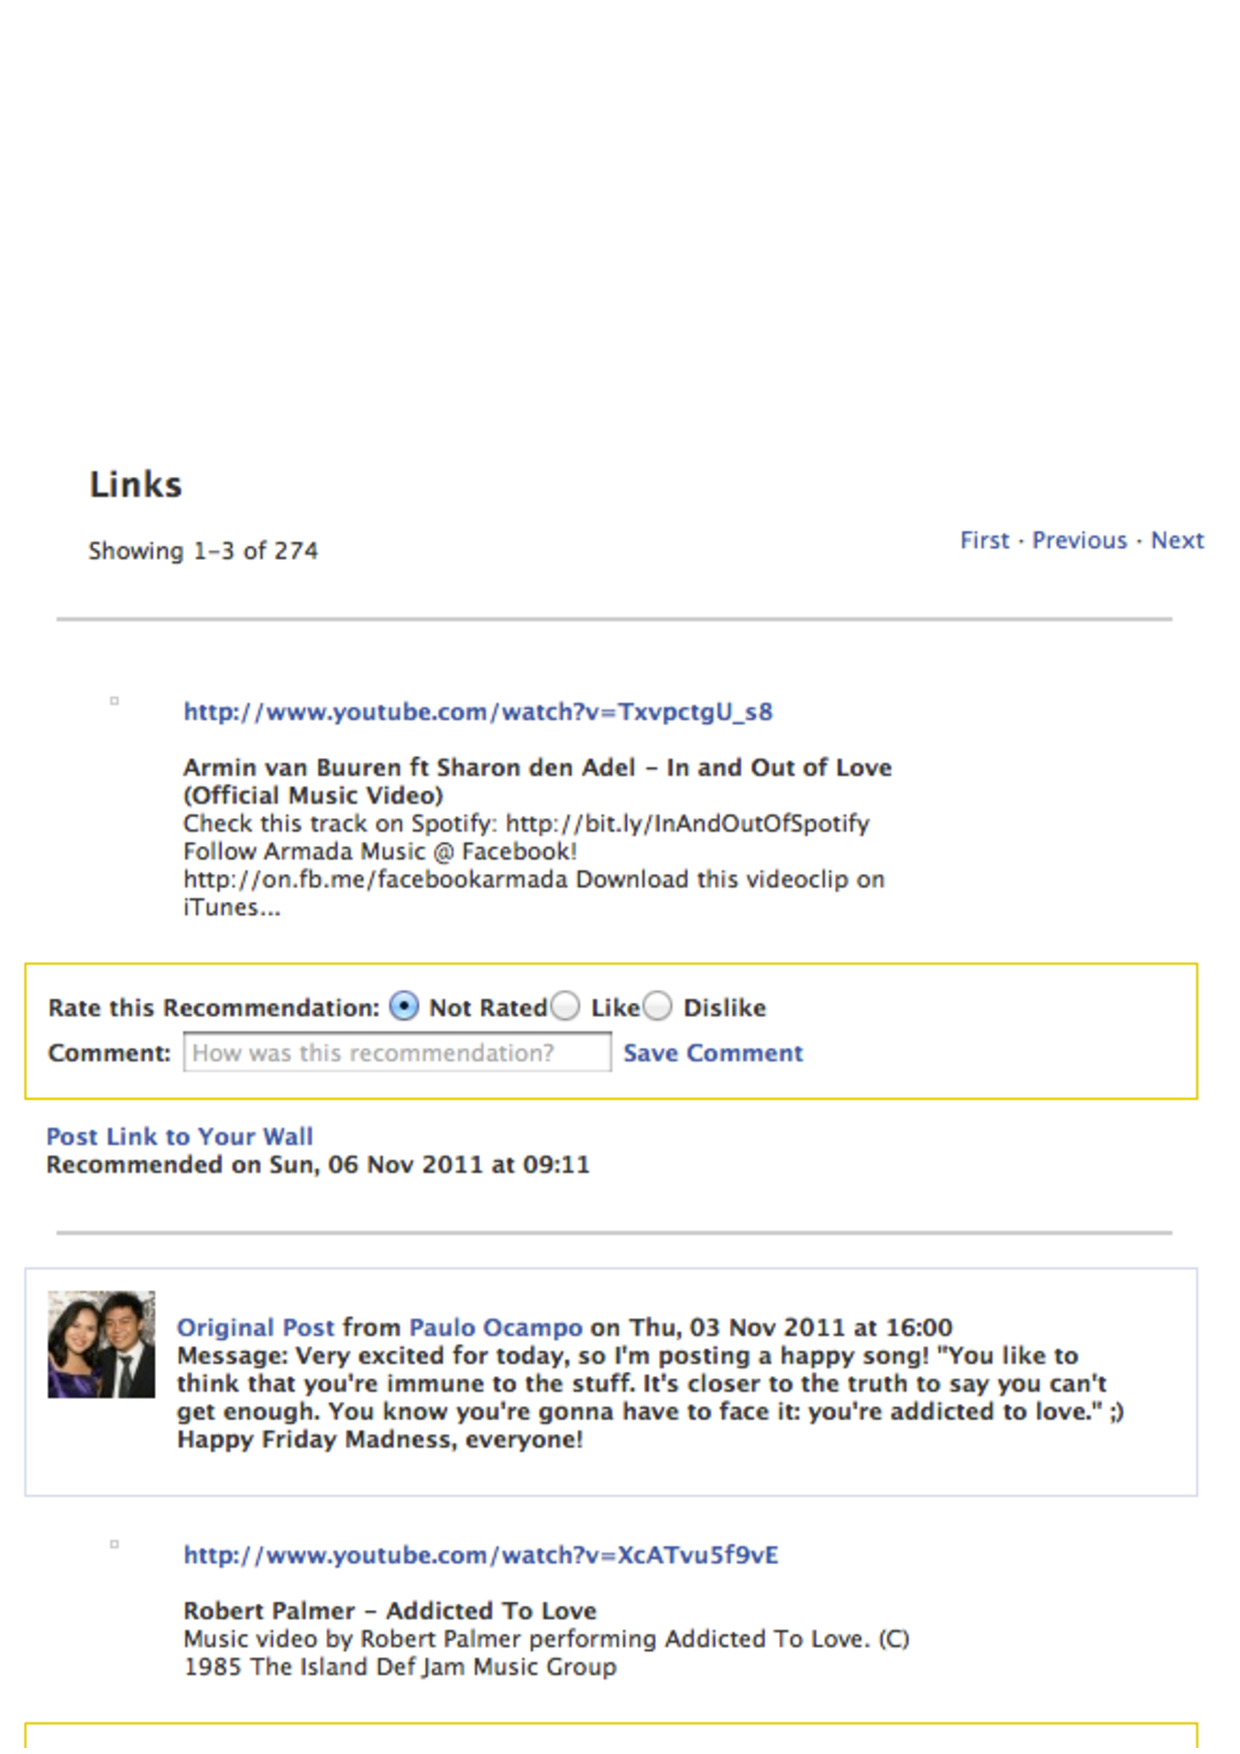
\includegraphics[scale=0.30]{img/linkr.png}}
\hspace{-2mm} \subfigure{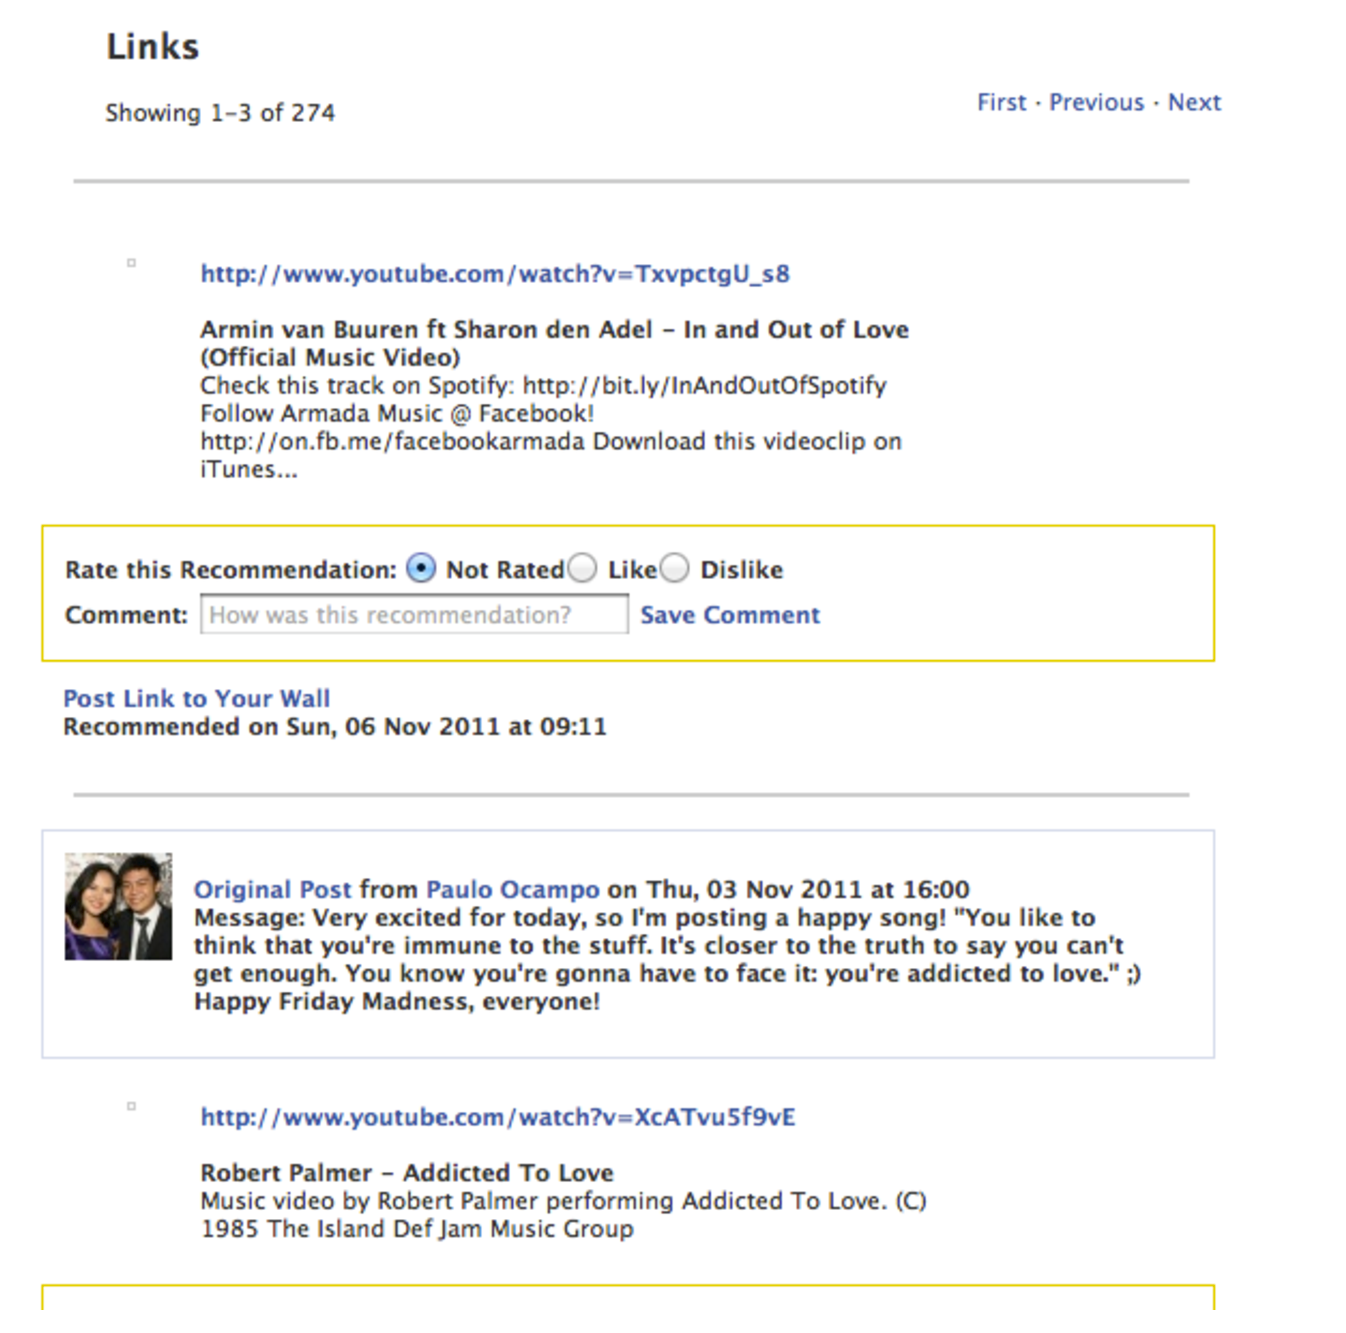
\includegraphics[scale=0.42]{img/linkr.eps}}
\caption{The Facebook LinkR App showing one of the recommendations
as it appears to users of the system.  Users have the option of liking
or disliking a recommendation as well as providing explicit feedback
commentary.}
\label{fig:linkr_app}
\end{figure}

\subsection{Dataset}

\label{sec:dataset}

Using the LinkR Facebook App developed for this project, we were able
to gather data on 34,860 users and 437,023 links.

\subsubsection{User Data}

Date that are collected and used for the user features are as follows:
\begin{itemize}
\item {Gender:} male or female
\item {Birthday:} year
\item {$\mathit{location}_\mathit{id}$:} an integer ID corresponding
to the user's specific present location (city and country)
\item {$\mathit{hometown}_\mathit{id}$:} an integer ID corresponding
to the user's specific home town (city and country)
\item {$F_{\x,\z} \in \{ 0, 1\}$:} indicator of whether 
users $\x$ and $\z$ are friends.
% Joseph: be specific here...
\item {$\mathit{Int}_{\x,\z} \in \mathbb{N}$:} interactions on
Facebook between users $\x$ and $\z$ as defined in Section~\ref{sec:notation}.
\end{itemize}

\subsubsection{Link Data}

Data that are used for the link features are:
\begin{itemize}
\item{$\mathit{id}$ of the user who posted the link.}
\item{$\mathit{id}$ of the user on whose wall the link was posted.}
\item{Text description of the link from the user who posted it.}
\item{Text link summary from the metatags on the target link webpage.}
\item{Number of times the link has been liked.}
\item{Number of times the link has been shared.}
\item{Number of comments posted on the link}.
\item {$F'_{\x,\y} \in \{0, 1\}$:} indicator of whether user $\x$ has liked item $\y$.
\end{itemize}
Additionally, links that have been recommended by the LinkR
application have the following extra features:
\begin{itemize}
\item{$\mathit{id}$'s of users who have clicked on the link url.}
\item{Optional ``Like'' or ``Dislike'' rating of the LinkR user on the link.}
\end{itemize}

\subsubsection{Interaction Data}
\label{sec:interactions}

The interactions between users that we count (equally weighted) to define
$\mathit{Int}_{\x,\z}$ are:

\begin{enumerate}
\item{Being friends.}
\item{Posting an item (link, photo, video, photo, or message) on a user's wall.}
\item{Liking an item (link, photo, video, photo, or message) on a user's wall.}
\item{Commenting on an item (link, photo, video, photo, or message) on a user's wall.}
\item{Being tagged together in the same photo.}
\item{Being tagged together in the same video.}
\item{Two users tagging themselves as attending the same school.}
\item{Two users tagging themselves as attending the same class in school.}
\item{Two users tagging themselves as playing sports together.}
\item{Two users tagging themselves as working together for the same company.}
\item{Two users tagging themselves as working together on the same project for the same company.}
\end{enumerate}

\subsubsection{Live Online Recommendation Trials}

For the recommendations made to the LinkR application users, we select
only links posted in the most recent two weeks that the user has not
liked. We use only the links from the last two weeks since an informal
user study has indicated a preference for recent links.  Furthermore,
older links have a greater chance of being outdated and are also
likely to represent broken links that are not working anymore. We have
settled on recommending three links per day to the LinkR users and
according to the survey done at the end of the first trial, three
links per day seems to be the generally preferred number of
daily recommendations.

For the live trials, Facebook users who installed the LinkR
application were \emph{randomly assigned one of four algorithms in
each of the two trials}. Users were not informed which algorithm was
assigned to them to remove any bias. We distinguish our recommended
links into two major classes, links that were posted by the LinkR
user's friends and links that were posted by users other than the
LinkR user's friends. The LinkR users were encouraged to rate the
links that were recommended to them, and even provide feedback
comments on the specific links. In turn these ratings became part of
the training data for the recommendation algorithms, and thus were used
to improve the performance of the algorithms over time. Based on the
user feedback, we filtered out non-English links and links without any
descriptions from the recommendations to prevent user annoyance.

At the end of the first trial, we conducted a user survey with the
LinkR users to find out how satisfied they were with the
recommendations they were getting.
 